% -*- mode: LaTeX; TeX-PDF-mode: t; -*- # Tell emacs the file type (for syntax)
% Add the listed directories to the search path
% (allows easy moving around later)
% warning: these paths are searched AFTER local config kpsewhich
\makeatletter
\def\input@path{{./.resources/latex/}{./.resources/texmf-local/tex/latex}{./resources/texmf-local/tex/bibtex}{./.resources/econ-ark}{./Resources/LaTeXInputs/}{./Resources/texmf-local/tex/latex/}}
\makeatother 

\documentclass[titlepage, headings=optiontotocandhead]{econtex}
\newcommand{\texname}{cctwMoM} % Keyname for the paper
%\usepackage{./.econtexRoot}         % Set paths (like, \LaTeXInputs)

\usepackage{local-macros}   % defns for this project
\usepackage{econark}        % econark defns
\usepackage{local-packages} % LaTeX config in .resources/LaTeXInputs
\usepackage{cctwMoM}        % LaTeX config in .resources/LaTeXInputs

% Switches
% Controls for which of various variant versions to create

\provideboolean{ctwVersion}\setboolean{ctwVersion}{false}\newcommand{\ctw}{\ifthenelse{\boolean{ctwVersion}}} % {cctw}
\provideboolean{trpVersion}\setboolean{trpVersion}{false}\newcommand{\trp}{\ifthenelse{\boolean{trpVersion}}} % {trp}
% \setboolean{trpVersion}{true} % {trp}
\setboolean{trpVersion}{false} % {trp}

% Draft mode puts \labels of figs, tables, eqns in margin
\provideboolean{draftmode}\setboolean{draftmode}{true}
% \setboolean{draftmode}{false}
\newcommand{\Draft}{\ifthenelse{\boolean{draftmode}}}

\Draft{\usepackage{showlabels}
  \renewcommand{\showlabelsetlabel}[1]{\tiny #1}
}{}

% RiskyR
\provideboolean{RiskyR}
\setboolean{RiskyR}{true}
\setboolean{RiskyR}{false}
\newcommand{\IfRiskyR}{\ifthenelse{\boolean{RiskyR}}}

% Include or exclude Method of Moderation material 
\provideboolean{MoMVersion}\setboolean{MoMVersion}{true}
%\setboolean{MoMVersion}{false}
\newcommand{\MoM}{\ifthenelse{\boolean{MoMVersion}}}

% Get extra style stuff for cctwMoM
\MoM{ % {cctw}
  \usepackage{cctwMoM} % {cctw}
}{} % {cctw}

% Versions with or without permanent shocks
% Seems to be defunct - remove
\provideboolean{PermShkVersion}\setboolean{PermShkVersion}{true}
\setboolean{PermShkVersion}{false}
\newcommand{\PermShkOn}{\ifthenelse{\boolean{PermShkVersion}}}

% MPCMatch version does Hermite polynomials for the interpolation
% that match both the slope and the intercept at the gridpoints
\provideboolean{MPCMatchVersion}
\setboolean{MPCMatchVersion}{true}
\newcommand{\MPCMatch}{\ifthenelse{\boolean{MPCMatchVersion}}}

% margin notes -- to be deleted
\provideboolean{MyNotes}\setboolean{MyNotes}{true}
\setboolean{MyNotes}{false} 

% Show things that need fixing
\provideboolean{ToFix}\setboolean{ToFix}{true}
% \setboolean{ToFix}{false} 
\newcommand{\Fix}{\ifthenelse{\boolean{ToFix}}}

 % booleans that control whether certain features are on or off

\hypersetup{colorlinks=true,
  pdfauthor={Christopher D. Carroll <ccarroll@jhu.edu>, Kiichi Tokuoka <ktokuoka <ktokuoka@imf.org>, Weifeng Wu <wwu19@jhu.edu> },
  pdftitle={The Method of Moderation},
  pdfsubject={Dynamic Stochastic Optimization Theory; Lecture Notes},
  pdfkeywords={Numerical Methods, Software},
  pdfproducer = {LaTeX with hyperref and thumbpdf},
  pdfcreator = {pdflatex}
}

\begin{verbatimwrite}{./\texname.title}
  The Method of Moderation
\end{verbatimwrite}

\bibliographystyle{econtex}
\begin{document}

% Redefine \onlyinsubfile command defined in local.sty file:
% This lets any submaterial called from here know that it is not standalone
% If not called from here and IS standalone, can make bib (or other content)
\renewcommand{\onlyinsubfile}[1]{}\renewcommand{\notinsubfile}[1]{#1}

\title{The Method of Moderation}

\author{Christopher D. Carroll\num \\ {\small JHU}
  \and
  Karsten Chipeniuk \\ {\small RBNZ}
  \and 
  Kiichi Tokuoka\num \\ {\small ECB}
  \and
  Weifeng Wu\num \\ {\small Fannie Mae}
}

\keywords{Dynamic Stochastic Optimization}
\jelclass{FillInLater}

\maketitle

\hypertarget{abstract}{}
\begin{abstract}
  In a risky world, a pessimist assumes the worst will happen.  Someone who ignores risk altogether is an optimist.  Consumption decisions are mathematically simple for both the pessimist and the optimist because both behave as if they live in a riskless world.  A realist (someone who wants to respond optimally to risk) faces a much more difficult problem, but (under standard conditions) will choose a level of spending somewhere between pessimist's and the optimist's.  We use this fact to redefine the space in which the realist searches for optimal consumption rules.  The resulting solution accurately represents the numerical consumption rule over the entire interval of feasible wealth values with remarkably few computations.
\end{abstract}

% \begin{small}
%   \parbox{\textwidth}{
%   \begin{center}
%     \begin{tabbing}
%       \texttt{Archive:~} \= \= \url{http://econ.jhu.edu/people/ccarroll/papers/ctwMoM.pdf} \kill \\  % This line establishes the locations of the tabs, but is not printed because of the \kill directive
%       \texttt{~~~~PDF:~} \> \> \url{http://econ.jhu.edu/people/ccarroll/papers/ctwMoM.pdf} \\
%       \texttt{~Slides:~} \> \> \url{http://econ.jhu.edu/people/ccarroll/papers/ctwMoM-Slides.pdf} \\
%       \texttt{~~~~Web:~} \> \> \url{http://econ.jhu.edu/people/ccarroll/papers/ctwMoM/} \\
%       \texttt{Archive:~} \> \> \url{http://econ.jhu.edu/people/ccarroll/papers/ctwMoM.zip} \\
% %       \texttt{~~~~~~~~~} \> \> \textit{(Contains data and estimation software producing paper's results)}
%     \end{tabbing}
%   \end{center}
% }
% \end{small}

\begin{authorsinfo}
  \name{Carroll: Department of Economics, Johns Hopkins University, Baltimore, MD, \url{http://econ.jhu.edu/people/ccarroll/}, \href{mailto:ccarroll@jhu.edu}{\texttt{ccarroll@jhu.edu}}}
  \name{Tokuoka: International Monetary Fund, Washington, DC, \href{mailto:ktokuoka@imf.org}{\texttt{ktokuoka@imf.org}}}
  \name{Wu: Weifeng Wu, Fanie Mae, Washington DC, \href{mailto:weifeng\_wu@fanniemae.com}.}
\end{authorsinfo}

\thanks{The views presented in this paper are those of the authors, and should not be attributed to the International Monetary Fund, its Executive Board, or management, or to the European Central Bank.}

\thispagestyle{empty}


\pagebreak\newpage

%\renewcommand{\DiscAlt}{\beta} % Erase the distinction between the alternative and the standard discount factor

\hypertarget{introduction}{}
\section{Introduction}\label{sec:Intro}

Solving a consumption, investment, portfolio choice, or similar intertemporal optimization problem using numerical methods generally requires the modeler to choose how to represent a policy or value function.  In the stochastic case, where analytical solutions are generally not available, a common approach is to use low-order polynominal splines that exactly match the function (and maybe some derivatives) at a finite set of gridpoints, and then to assume that interpolated or extrapolated versions of that spline represent the function well at the continuous infinity of unmatched points.

This paper argues that a better approach in the standard consumption problem is to rely upon the fact that without uncertainty, the optimal consumption function has a simple analytical solution.  The key insight is that, under standard assumptions, the consumer who faces an uninsurable labor income risk will consume less than a consumer with the same path for expected income but who does not perceive any uncertainty as being attached to that future income.  The `realistic' consumer, who \textit{ does} perceive the risks, will engage in `precautionary saving,' so the perfect foresight riskless solution provides an upper bound to the solution that will actually be optimal.  A lower bound is provided by the behavior of a consumer who has the subjective belief that the future level of income will be the worst that it can possibly be.  This consumer, too, behaves according to the convenient analytical perfect foresight solution, but his certainty is that of a pessimist perfectly confident in his pessimism.

Using results from \cite{BufferStockTheory}, we show how to use these upper and lower bounds to tightly constrain the shape and characteristics of the solution to problem of the `realist.'  Imposition of these constraints can clarify and speed the solution of the realist's problem.

After showing how to use the method in the baseline case, we show how refine it to encompass an even tighter theoretical bound\IfRiskyR{, and how to extend it to solve a problem in which the consumer faces both labor income risk and rate-of-return risk.}{.}

\hypertarget{the-realists-problem}{}
\section{The Realist's Problem}

We assume that truly optimal behavior in the problem facing the consumer who understands all his risks is captured by
  \begin{equation}\label{eq:MaxProb}
    \max ~ \Ex_{t}\left[ \sum_{n_{\TranShkEmp}=0}^{T-t} {\DiscAlt}^{n_{\TranShkEmp}} \uFunc({\cLvl}_{t+n})\right],
  \end{equation}

\notinsubfile{\input{./.resources/latex/bibliography-blend}} \end{document}\endinput
subject to
  \begin{equation}\begin{gathered}\begin{aligned}
        \aLvl_{t}  & = \mLvl_{t}-\cLvl_{t} \label{DBCLevel}%\label{DBCLevelStart}
        \\  {\bLvl}_{t+1}  & = \aLvl_{t} \Rfree_{t+1}
        \\  {\yLvl}_{t+1}  & = \pLvl_{t+1}\TranShkEmp_{t+1}
        \\  \mLvl_{t+1}  & = {\bLvl}_{t+1} + {\yLvl}_{t+1} %\label{DBCLevelEnd}
      \end{aligned}\end{gathered}\end{equation}

where
  \begin{equation*}\begin{gathered}\begin{aligned}
        {\DiscAlt}  & - \text{pure time discount factor} \\
        \aLvl_{\prdt}  & - \text{assets after all actions have been accomplished in period $t$} \\
        \cLvl_{\prdt}  & - \text{consumption in period $t$} \\
        \mLvl_{\prdt}  & - \text{`market resources' available for consumption (`cash-on-hand')} \\
        \pLvl_{\prdt+1}  & - \text{`permanent labor income' in period $t+1$} \\
        \Rfree_{\prdt+1}  & - \text{interest factor $(1+\rfree_{\prdt+1})$ from period $t$ to $t+1$ } \\
        \yLvl_{\prdt+1}  & - \text{noncapital income in period $t+1$}.
      \end{aligned}\end{gathered}\end{equation*}

and the exogenous variables evolve according to 
  \begin{equation}\begin{gathered}\begin{aligned}
        \pLvl_{\prdt+1}   = \PermGroFac_{\prdt+1}\pLvl_{\prdt}                                        & \text{~~ -- permanent labor income dynamics} \label{eq:permincgrow}
        \\ \log ~ \tranShkEmp_{\prdt+n}  \sim ~\Nrml(-\std_{\tranShkEmp}^{2}/2,\std_{\tranShkEmp}^{2}) & \text{~~ -- lognormal transitory shocks}~\forall~n>0 .
        %
        \UnifiedNote{Shock space 𝒵ₐᵥ definition; ζₐᵥ = (ψ, θ) with distributions Pₐᵥ}
      \end{aligned}\end{gathered}\end{equation}


It turns out (see \cite{SolvingMicroDSOPs} for a proof) that this problem can be rewritten in a more convenient form in which choice and state variables are normalized by the level of permanent income, e.g., using nonbold font for normalized variables, $\mNrm_{t}=\cLvl_{t}/\pLvl_{t}$.  When that is done, the Bellman equation for the transformed version of the consumer's problem is \begin{eqnarray}
        \null{\vFunc}_{t}({m}_{t}) & = & \max_{{c}_{t}} ~~ \util({c}_{t})+
        \Ex_{t}[{\Discount} \PGro_{t+1}^{1-\CRRA}\null{\vFunc}_{t+1}({m}_{t+1})] \label{vtNorm}
\\         & \text{s.t.} &   \nonumber \\
    {a}_{t}   & = & {m}_{t}-{c}_{t} \nonumber
\\      {m}_{t+1} & = & \underbrace{\left(\Rfree/\PGro_{t+1}\right)}_{\equiv \Rnorm_{t+1}}{a}_{t}+\tShkEmp_{t+1} \nonumber
\end{eqnarray}
 and because we have not imposed a liquidity constraint, the solution satisfies the Euler equation   \begin{equation}\begin{gathered}\begin{aligned}
        \uFunc^{\partial}(\cNrm_{\prdt})  & = \ExEndPrd[\DiscFac \Rfree \PermGroFac_{\prdt+1}^{-\CRRA}\uFunc^{\partial}(\cNrm_{\prdt+1})] \label{eq:cEuler}.
        %
        \UnifiedNote{Euler equation (combines envelope + FOC across periods)}
      \end{aligned}\end{gathered}\end{equation}


For the remainder of the paper we will assume that permanent income $\pLvl_{t}$ grows by a constant factor $\PermGroFac$ and is not subject to stochastic shocks.  (The generalization to the case with permanent shocks is straightforward.)

\hypertarget{benchmark}{}
\section{Benchmark: The Method of Endogenous Gridpoints}

For comparison to our new solution method, we use the endogenous gridpoints solution to the microeconomic problem presented in \cite{carrollEGM}.  That method computes the level of consumption at a set of gridpoints for market resources $\mNrm$ that are determined endogenously using the Euler equation.  The consumption function is then constructed by linear interpolation among the gridpoints thus found.

\cite{SolvingMicroDSOPs} describes a specific calibration of the model and constructs a solution using five gridpoints chosen to capture the structure of the consumption function reasonably well at values of $\mNrm$ near the infinite-horizon target value.  (See those notes for details).


  Unfortunately, this endogenous gridpoints solution is not very
  well-behaved outside the original range of gridpoints targeted by
  the solution method.  (Though other common solution methods are no
  better outside their own predefined ranges).
  Figure~\ref{fig:ExtrapProblem} demonstrates the point by plotting
  the amount of precautionary saving implied by a linear extrapolation
  of our approximated consumption rule (the consumption of the perfect
  foresight consumer $\cFuncAbove_{T-1}$ minus our approximation to
  optimal consumption under uncertainty, $\Alt{\cFunc}_{T-1}$).
  Although theory proves that precautionary saving is always positive,
  the linearly extrapolated numerical approximation eventually
  predicts negative precautionary saving (at the point in the figure
  where the extrapolated locus crosses the horizontal axis).

\hypertarget{ExtrapProblemPlot}{}
\begin{figure}
        \includegraphics{./Figures/ExtrapProblemPlot}
        \caption{For Large Enough ${m}_{T-1}$, Predicted Precautionary Saving is Negative (Oops!)}
        \label{fig:ExtrapProblem}
\end{figure}

This error cannot be fixed by extending the upper gridpoint; in the
presence of serious uncertainty, the consumption rule will need to be
evaluated outside of \textit{any} prespecified grid (because starting
from the top gridpoint, a large enough realization of the uncertain
variable will push next period's realization of assets above that
top; a similar argument applies below the bottom gridpoint).  While a judicious extrapolation technique can prevent this
problem from being fatal (for example by carefully excluding negative
precautionary saving), the problem is often dealt with using inelegant
methods whose implications for the accuracy of the solution are
difficult to gauge.


\hypertarget{the-method-of-moderation}{}
\section{The Method of Moderation}

\hypertarget{the-optimist-the-pessimist-and-the-realist}{}
\subsection{The Optimist, the Pessimist, and the Realist}

\hypertarget{the-consumption-function}{}
\subsubsection{The Consumption Function}

\begin{verbatimwrite}{./cctwMoM/MoM-Prelims.tex}
  As a preliminary to our solution, define $\hNrm_{\EndStg}$ as end-of-period human wealth (the present discounted value of future labor income) for a perfect foresight version of the problem of a `risk optimist:' a period-$t$ consumer who believes with perfect confidence that the shocks will always take their expected value of \PermShkOn{1, $\TranShkEmp_{t+n} = \Ex[\TranShkEmp]=1~\forall~n>0$ and $\permShk_{t+n} = \Ex[\permShk]=1~\forall~n>0$.}{1, $\TranShkEmp_{t+n} = \Ex[\TranShkEmp]=1~\forall~n>0$.}  The solution to a perfect foresight problem of this kind takes the form\footnote{For a derivation, see \cite{BufferStockTheory}; $\MPCmin_{t}$ is defined therein as the MPC of the perfect foresight consumer with horizon $T-t$.}
\end{verbatimwrite}
As a preliminary to our solution, define $\hEnd_{t}$ as
end-of-period human wealth (the present discounted value
of future labor income) for a perfect foresight version of the problem
of a `risk optimist:' a consumer who believes with perfect confidence
that the shocks will always take the value
\pShkOn
{1, $\tShkEmp_{t+n} = \Ex[\tShkEmp]=1~\forall~n>0$ and $\pShk_{t+n} = \Ex[\pShk]=1~\forall~n>0$.}
{1, $\tShkEmp_{t+n} = \Ex[\tShkEmp]=1~\forall~n>0$.}
The solution to a perfect foresight problem of this kind takes the
form\footnote{For a derivation, see \cite{BufferStockTheory}; $\MinMPC_{t}$ is defined therein as the MPC of the perfect foresight consumer with horizon $T-t$.}
\unskip
\begin{verbatimwrite}{./Equations/cFuncAbove.tex}
  \begin{equation}\begin{gathered}\begin{aligned}
        \cFuncAbove_{t}(\mNrm_{t})  & = (\mNrm_{t} + \hNrm_{\EndStg})\MPCmin_{t} \label{eq:cFuncAbove}
      \end{aligned}\end{gathered}\end{equation}
  for a constant minimal marginal propensity to consume $\MPCmin_{t}$ given below.
\end{verbatimwrite}
  \begin{equation}\begin{gathered}\begin{aligned}
        \cFuncAbove_{\prd}(\mNrm_{\prd})  & = (\mNrm_{\prd} + \hNrm_{\Cntn})\MPCmin_{\prd} \saferlabel{eq:cFuncAbove} % Don't define it if already defined
        %
        \UnifiedNote{[no direct counterpart] (computational: upper-bound perfect foresight consumption rule for MoM)}
      \end{aligned}\end{gathered}\end{equation}
  for a constant minimal marginal propensity to consume $\MPCmin_{\prd}$ given below.
\unskip

  \begin{equation}\begin{gathered}\begin{aligned}
        \cFuncAbove_{\prd}(\mNrm_{\prd})  & = (\mNrm_{\prd} + \hNrm_{\Cntn})\MPCmin_{\prd} \saferlabel{eq:cFuncAbove} % Don't define it if already defined
        %
        \UnifiedNote{[no direct counterpart] (computational: upper-bound perfect foresight consumption rule for MoM)}
      \end{aligned}\end{gathered}\end{equation}
  for a constant minimal marginal propensity to consume $\MPCmin_{\prd}$ given below.
 
  We similarly define $\hEndMin_{t}$ as `minimal human wealth,' the
  present discounted value of labor income if the shocks were to take on
  their worst possible value in every future period \PermShkOn
  {$\TranShkEmp_{t+n} = \TranShkEmpMin ~\forall~n>0$ and $\PermShk_{t+n} =
    \PermShkMin ~\forall~n>0$} {$\TranShkEmp_{t+n} = \TranShkEmpMin
    ~\forall~n>0$} (which we define as corresponding to the beliefs of a
  `pessimist').

  \ctw{}{We will call a `realist' the consumer who correctly perceives the true
    probabilities of the future risks and optimizes accordingly.}

  A first useful point is that, for the realist, a lower bound for the
  level of market resources is $\ushort{m}_{t} = -\hEndMin_{t}$, because
  if ${m}_{t}$ equalled this value then there would be a positive finite
  chance (however small) of receiving \PermShkOn
  {$\TranShkEmp_{t+n}=\TranShkEmpMin$ and $\PermShk_{t+n}=\PermShkMin$}
  {$\TranShkEmp_{t+n}=\TranShkEmpMin$}
  in
  every future period, which would require the consumer to set ${c}_{t}$
  to zero in order to guarantee that the intertemporal budget constraint
  holds\ctw{.}{~(this is the multiperiod generalization of the discussion in
    section \ref{subsec:LiqConstrSelfImposed} about
    $\ushort{a}_{T-1}$).}  Since consumption of zero yields negative
  infinite utility, the solution to realist consumer's problem is not well
  defined for values of ${m}_{t} < \ushort{m}_{t}$, and the limiting
  value of the realist's ${c}_t$ is zero as ${m}_{t} \downarrow \ushort{m}_{t}$.

  Given this result, it will be convenient to define `excess' market
  resources as the amount by which actual resources exceed the lower
  bound, and `excess' human wealth as the amount by which mean expected human wealth
  exceeds guaranteed minimum human wealth:
  \begin{equation*}\begin{gathered}\begin{aligned}
        \aboveMin \mNrm_{t}  & = {m}_{t}+\overbrace{\hEndMin_{t}}^{=-\ushort{m}_{t}}
        \\  \aboveMin \hEnd_{t}  & = \hEnd_{t}-\hEndMin_{t}.
      \end{aligned}\end{gathered}\end{equation*}

  We can now transparently define the optimal
  consumption rules for the two perfect foresight problems, those of the
  `optimist' and the `pessimist.'  The `pessimist' perceives human
  wealth to be equal to its minimum feasible value $\hEndMin_{t}$ with certainty, so
  consumption is given by the perfect foresight solution
  \begin{equation*}\begin{gathered}\begin{aligned}
        \cFuncBelow_{t}(m_{t})  & = ({m}_{t}+\hEndMin_{t})\MPCmin_{t}
        \\  & = \aboveMin \mNrm_{t}\MPCmin_{t}
        .
      \end{aligned}\end{gathered}\end{equation*}

  The `optimist,' on the other hand, pretends that there is no uncertainty
  about future income, and therefore consumes
  \begin{equation*}\begin{gathered}\begin{aligned}
        \cFuncAbove_{t}(m_{t})  & = ({m}_{t} +\hEndMin_{t} - \hEndMin_{t} + \hEnd_{t} )\MPCmin_{t}
        \\    & = (\aboveMin \mNrm_{t} + \aboveMin \hEnd_{t})\MPCmin_{t}
        \\      & = \cFuncBelow_{t}(m_{t})+\aboveMin \hEnd_{t} \MPCmin_{t}
        .
      \end{aligned}\end{gathered}\end{equation*}

  It seems obvious that the spending of the realist will be strictly greater
  than that of the pessimist and strictly less than that of the
  optimist.  Figure~\ref{fig:IntExpFOCInvPesReaOptNeedHiPlot} illustrates the proposition for the consumption rule in period $T-1$.


\import{./Figures/}{IntExpFOCInvPesReaOptNeedHiPlot.tex}


  \indent Proof is more difficult than might be imagined, but
the necessary work is done in \cite{BufferStockTheory} so we will take
the proposition as a fact and proceed by manipulating the inequality:

\begin{center}
	\begin{tabular}{rcl}
		$  \cFuncBelow_{t}(m_{t}) = \aboveMin \mNrm_{t} \MPCmin_{t} < $ & $ \cFunc_{t}(\ushort{m}_{t}+\aboveMin \mNrm_{t}) $ & $< (\aboveMin \mNrm_{t}+\aboveMin \hEnd_{t})\MPCmin_{t} = $ $ \bar{\cFunc}_{t}(\ushort{m}_{t}+\aboveMin \mNrm_{t})$
		%      \\  $- \aboveMin \mNrm_{t} \MPCmin_{t} > $ & $ -\cFunc_{t}(\ushort{m}_{t}+\aboveMin \mNrm_{t}) $ & $> -(\aboveMin \mNrm_{t}+\aboveMin \hEnd_{t})\MPCmin_{t} $
		%      \\  $ \aboveMin \hEnd_{t} \MPCmin_{t} > $ & $ \bar{\cFunc}_{t}(\ushort{m}_{t}+\aboveMin \mNrm_{t})-\cFunc_{t}(\ushort{m}_{t}+\aboveMin \mNrm_{t}) $ & $> 0$
		%      \\  $1 > $ & $ \underbrace{\left(\frac{\bar{\cFunc}_{t}(\ushort{m}_{t}+\aboveMin \mNrm_{t})-\cFunc_{t}(\ushort{m}_{t}+\aboveMin \mNrm_{t})}{\aboveMin \hEnd_{t} \MPCmin_{t}}\right)}_{\equiv \Hi{\koppa}_{t}} $ & $> 0$
	\end{tabular}
\end{center}

where the fraction in the middle of the last inequality is the ratio
of actual precautionary saving (the numerator is the difference
between perfect-foresight consumption and optimal consumption in the
presence of uncertainty) to the maximum conceivable amount of
precautionary saving (the amount that would be undertaken by the
pessimist who consumes nothing out of any future income beyond the perfectly certain component).

  Defining $\mu_{\prdt} =
  \log \aboveMin \mNrm_{\prdt}$ (which can range from $-\infty$ to $\infty$), the object in the middle of the last inequality is
  \begin{equation}\begin{gathered}\begin{aligned}
        \Max{\koppa}_{\prdt}(\mu_{\prdt})   & \equiv  \left(\frac{\bar{\cFunc}_{\prdt}(\Min{m}_{\prdt}+e^{\mu_{\prdt}})-\cFunc_{\prdt}(\Min{m}_{\prdt}+e^{\mu_{\prdt}})}{\aboveMin \hNrm_{\Cntn} \MPCmin_{\prdt}}\right), \label{eq:koppa}
        %
        \UnifiedNote{[no direct counterpart] (computational: koppa — bounded interpolant between pessimist/optimist consumption)}
      \end{aligned}\end{gathered}\end{equation}
  and we now define
  \begin{equation}\begin{gathered}\begin{aligned}
        \Max{\chiFunc}_{\prdt}(\mu_{\prdt})  & = \log \left(\frac{1-\Max{\koppa}_{\prdt}(\mu_{\prdt})}{\Max{\koppa}_{\prdt}(\mu_{\prdt})}\right)
        \\  & = \log \left(1/\Max{\koppa}_{\prdt}(\mu_{\prdt})-1\right) \label{eq:chi}
        %
        \UnifiedNote{[no direct counterpart] (computational: chi — log-odds transform of koppa for interpolation)}
      \end{aligned}\end{gathered}\end{equation}

which has the virtue that it is linear in the limit as $\mu_{t}$ approaches $+\infty$.

Given $\Hi{\chiFunc}$, the consumption function can be recovered from

  \begin{equation}\begin{gathered}\begin{aligned}
    \Hi{\cFunc}_{t}  & = \bar{\cFunc}_{t}-\overbrace{\left(\frac{1}{1+\exp(\Hi{\chiFunc}_{t})}\right)}^{=\Hi{\koppa}_{t}} \aboveMin \hEnd_{t} \MinMPC_{t}. \label{eq:cFuncHi}
  \end{aligned}\end{gathered}\end{equation}


  Using these inequalities, we now construct another approximation of consumption function, $\tilde{\cFunc}_{t}({m}_{t})$, whose performance is better for points lying outside the original grid. Denote the largest and smallest points on that grid by $\bar{m}$ and $\underaccent{\bar}{m}$ respectively.  The above inequality then tells us that we have a limiting function $ \bar{\cFunc}_{t}(\ushort{m}_{t}+\aboveMin \mNrm_{t})$ for values of m, greater than $\bar{m}$, i.e., for values of $m_t > \bar{m} $  and $m_t \rightarrow \infty $, the behavior of $\tilde{\cFunc}_{t}({m}_{t})$ is anchored by $ \bar{\cFunc}_{t}({m}_{t})$. More precisely, our improved consumption function's behavior would be governed by following  rules:
\begin{itemize}
\item $\tilde{\cFunc}_{t}({m}_{t})$  = $ \cFunc_{t}({m}_{t})$ when $m_t$ falls inside the specified grid, i.e.\ when $m_t$ < $\bar{m}$
\item $\tilde{\cFunc}_{t}({m}_{t})  \rightarrow    \cFuncBelow_{t}(m_{t})  $  as $m_t \rightarrow 0$.
\item $\tilde{\cFunc}_{t}({m}_{t})  \rightarrow   \bar{\cFunc}_{t}({m}_{t}) $  as $m_t \rightarrow \infty$.
\end{itemize}

With the above principle in mind, start with a point $m$ beyond the specified grid, $m > \bar{m}$. Since the gridpoints in our case are one-dimensional, the point in the grid closest to $m$ is $\bar{m}$. This method first calculates a standardized distance between $m$ and $\bar{m}$ as:
\begin{align*}
  d(m, \bar{m}) & =  \left| \frac{m - \bar{m}}{\bar{m}} \right|
\end{align*}
and uses it to compute the combination between extrapolated value  $ \cFunc_{t}({m}_{t})$ and the limit-value $\bar{\cFunc}_{t}({m}_{t}) $ as :

\[  \tilde{\cFunc}_{t}({m}_{t}) = e^{-d(m, \bar{m})} \times   \cFunc_{t}({m}_{t})  +  (1-e^{-d(m, \bar{m})})\times  \bar{\cFunc}_{t}({m}_{t})\]

i.e. our improved approximation of consumption function is a weighted average of  $ \cFunc_{t}({m}_{t})$ and  $\bar{\cFunc}_{t}({m}_{t}) $. As the distance between $m$ and $\bar{m}$ grows,  $\bar{\cFunc}_{t}({m}_{t})$ is given more weight. That makes intuitive sense as $m$ being far outside the pre-specified grid point range corresponds to the case of a large realization of temporary shock. And that means, consumer would have enormous market resources at its disposal than usual, in which case its consumption behavior would closely follow that of an optimist (i.e. $\bar{\cFunc}_{t}({m}_{t})$).
Readers interested in alternative methods of extrapolation should refer this HARK \href{https://github.com/econ-ark/HARK/blob/master/examples/Interpolation/DecayInterp.ipynb}{documentation}.

So far, we have discussed the procedure to carry out extrapolation when the point is larger than the maximum grid point that was specified with $\bar{\cFunc}(m)$ as the benchmark function. By similar reasoning, we can also conduct extrapolation when the point is smaller than the minimum grid point with  $\cFuncBelow(m)$ serving now as the benchmark function anchoring the behavior of approximate consumption function in that point range.


  Because this method relies upon the fact that the problem is easy to
  solve if the decision maker has unreasonable views (either in the
  optimistic or the pessimistic direction), and because the correct
  solution is always between these immoderate extremes, we call our
  solution procedure the `method of moderation.'

  Results are shown in Figure~\ref{fig:ExtrapProblemSolved}; a reader
  with very good eyesight might be able to detect the barest hint of a
  discrepancy between the Truth and the Approximation at the far
  righthand edge of the figure\ctw{.}{ -- a stark contrast with the calamitous
    divergence evident in Figure~\ref{fig:ExtrapProblem}.}{}
  \hypertarget{ExtrapProblemSolvedPlot}{}
  \begin{figure}
    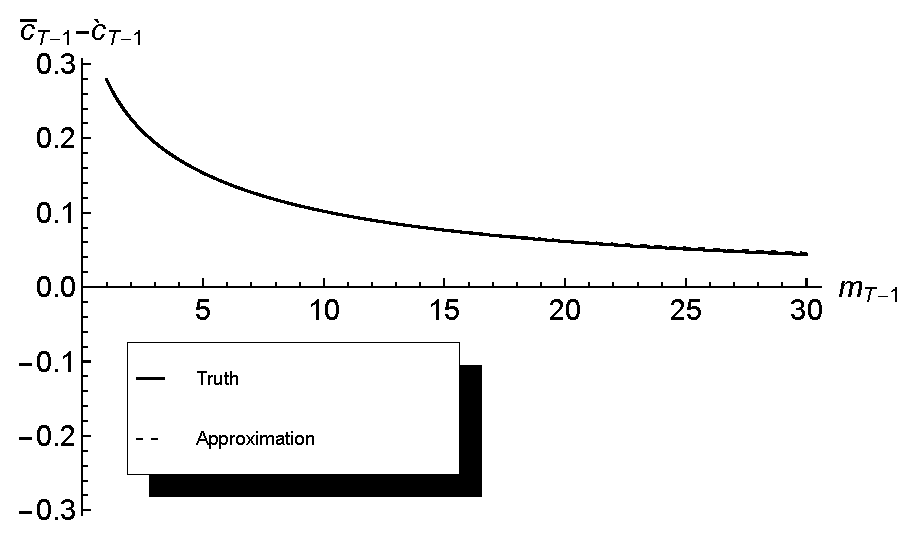
\includegraphics{./Figures/ExtrapProblemSolvedPlot}
    \caption{Extrapolated $\Alt{\Hi{\cFunc}}_{T-1}$ Constructed Using the Method of Moderation}
    \label{fig:ExtrapProblemSolved}
  \end{figure}



\hypertarget{the-value-function}{}
\subsubsection{The Value Function}


  Often it is useful to know the value function as well as the consumption rule.  Fortunately, many of the tricks used when solving for the consumption rule have a direct analogue in approximation of the value function.

  Consider the perfect foresight (or ``optimist's'') problem in period $\trmT-1$.  Using the fact that in a perfect foresight model the growth factor for consumption is $(\Rfree \DiscFac)^{1/\CRRA}$, we can use the fact that $\cNrm_{\prd} = (\Rfree \DiscFac)^{1/\CRRA} \cNrm_{\prd-1}$ to calculate the value function in period $\trmT-1$:
  \begin{equation*}\begin{gathered}\begin{aligned}
        \bar{\vFunc}_{\prd-1}({m}_{\prd-1})  & \equiv  \uFunc(\cNrm_{\prd-1})+\DiscFac \uFunc(\cNrm_{\prd})
        \\  & = \uFunc(\cNrm_{\prd-1})\left(1+\DiscFac ((\DiscFac\Rfree)^{1/\CRRA})^{1-\CRRA}\right)
        % \\  & = \uFunc(\cNrm_{\prd-1})\left(1+\DiscFac (\DiscFac\Rfree)^{1/\CRRA-1}\right)
        \\  & = \uFunc(\cNrm_{\prd-1})\left(1+(\DiscFac\Rfree)^{1/\CRRA}/\Rfree\right)
        \\  & = \uFunc(\cNrm_{\prd-1})\underbrace{\mbox{PDV}_{\prd}^{T}(\cNrm)/\cNrm_{\prd-1}}_{\equiv \PDVCoverc_{\prd-1}^{T}}
      \end{aligned}\end{gathered}\end{equation*}
  where $\PDVCoverc_{\prd}^{T}=\mbox{PDV}_{\prd}^{T}(\cNrm)$ is the present discounted value of consumption, normalized by current consumption. Using the fact demonstrated in \cite{BufferStockTheory} that $\PDVCoverc_{\prd}=\MPC^{-1}_{\prd}$, a similar function can be constructed recursively for earlier periods, yielding the general expression \hypertarget{vFuncPF}{}
 % Can't nest verbatimwrites so must split value.tex up into parts
  \begin{equation}\begin{gathered}\begin{aligned}
        \bar{\vFunc}_{\dcsn(\prdt)}(m_{\prdt})  & = \uFunc(\bar{\cNrm}_{\prdt})\PDVCoverc_{\prdt}^{T}\label{eq:vFuncPF}
        \\  & = \uFunc(\bar{c}_{\prdt}) \MPCmin_{\prdt}^{-1} % 20190820
        \\  & = \uFunc((\aboveMin \mNrm_{\prdt}+\aboveMin \hNrm_{\Cntn})\MPCmin_{\prdt}) \MPCmin_{\prdt}^{-1} % 20190820
        \\  & = \uFunc(\aboveMin \mNrm_{\prdt}+\aboveMin \hNrm_{\Cntn})\MPCmin_{\prdt}^{1-\CRRA} \MPCmin_{\prdt}^{-1} % 20190820
        \\  & = \uFunc(\aboveMin \mNrm_{\prdt}+\aboveMin \hNrm_{\Cntn})\MPCmin_{\prdt}^{-\CRRA}  % 20190820
        %
        \UnifiedNote{𝒱(xᵥ) (partial: upper-bound perfect foresight decision-value function for MoM)}
      \end{aligned}\end{gathered}\end{equation}

  This can be transformed as
  \begin{equation*}\begin{gathered}\begin{aligned}
        \bar{\vInv}_{\prdt}  & \equiv  \left((1-\CRRA)\bar{\vFunc}_{\dcsn(\prdt)}\right)^{1/(1-\CRRA)}
        \\  & = \cNrm_{\prdt}(\PDVCoverc_{\prdt}^{T})^{1/(1-\CRRA)}
        \\  & = (\aboveMin \mNrm_{\prdt}+\aboveMin \hNrm_{\Cntn})\MPCmin_{\prdt}^{-\CRRA/(1-\CRRA)}   % 20190820
      \end{aligned}\end{gathered}\end{equation*}
 % This is the perfect foresight solution 
\MPCMatch{with derivative
\begin{eqnarray*}
  \bar{\vInv}_{t}^{m} & = & (\mathbb{C}_{t}^{T})^{1/(1-\CRRA)}\MinMPC_{t},
\\ & = & \MinMPC_{t}^{-\CRRA/(1-\CRRA)} % 20190820
\end{eqnarray*}}{}
and since $\mathbb{C}_{t}^{T}$ is a constant while the consumption
function is linear, $\bar{\vInv}_{t}$ will also be linear.

We apply the same transformation to the value function for the problem with uncertainty (the ``realist's'' problem)\MPCMatch{ and differentiate}:
\begin{eqnarray*}
  \bar{\vInv}_{t} & = & \left((1-\CRRA)\bar{\vFunc}_{t}({m}_{t})\right)^{1/(1-\CRRA)}
\MPCMatch{\\ \bar{\vInv}^{m}_{t} & = & \left((1-\CRRA)\bar{\vFunc}_{t}({m}_{t})\right)^{-1+1/(1-\CRRA)}\bar{\vFunc}_{t}^{m}({m}_{t})}{}
\end{eqnarray*}
and an excellent approximation to the value function can be obtained by
calculating the values of $\bar{\vInv}$ at the same gridpoints used by the
consumption function approximation, and interpolating among those points.

However, as with the consumption approximation, we can do even better if we
realize that the $\bar{\vInv}$ function for the optimist's problem is
an upper bound for the ${\vInv}$ function in the presence of uncertainty, and the value function
for the pessimist is a lower bound. Analogously to \eqref{eq:koppa}, define an upper-case
\begin{eqnarray}
\hat{\Koppa}_{t}(\mu_{t})  & = & \left(\frac{\bar{\vInv}_{t}(\ushort{m}_{t}+e^{\mu_{t}})-\vInv_{t}(\ushort{m}_{t}+e^{\mu_{t}})}{\aboveMin \hEnd_{t} \MinMPC_{t} (\mathbb{C}_{t}^{T})^{1/(1-\CRRA)}}\right) \label{eq:Koppa}
\end{eqnarray}
\MPCMatch{with derivative (dropping arguments)
\begin{eqnarray}
 \hat{\Koppa}_{t}^{\mu}  & = & (\aboveMin \hEnd_{t} \MinMPC_{t} (\mathbb{C}_{t}^{T})^{1/(1-\CRRA)})^{-1}e^{\mu_{t}}\left(\bar{\vInv}^{m}_{t}-\vInv^{m}_{t}\right) \label{eq:KoppaPrime}
%\\ & = &  (\aboveMin \hEnd_{t} \MinMPC_{t})^{-1}e^{\mu_{t}}\left((\mathbb{C}_{t}^{T})^{1/(1-\CRRA)}\MinMPC_{t}-\left((1-\CRRA)\vFunc_{t}({m}_{t})\right)^{-1+1/(1-\CRRA)}\vFunc_{t}^{m}({m}_{t})\right)  \notag
\end{eqnarray}}{}
and an upper-case version of the $\chiFunc$ equation in \eqref{eq:chi}:
\begin{eqnarray}
  \hat{\Chi}_{t}(\mu_{t}) & = & \log \left(\frac{1-\hat{\Koppa}_{t}(\mu_{t})}{\hat{\Koppa}_{t}(\mu_{t})}\right)
\\ & = & \log \left(1/\hat{\Koppa}_{t}(\mu_{t})-1\right) \label{eq:Chi}
\end{eqnarray}
\MPCMatch{with corresponding derivative
\begin{eqnarray}
 \hat{\Chi}_{t}^{\mu} & = & \left(\frac{-\hat{\Koppa}_{t}^{\mu}/\hat{\Koppa}_{t}^{2}}{1/\hat{\Koppa}_{t}-1}\right)
\end{eqnarray}}{}
and if we approximate these objects then invert them (as above with
the $\Hi{\koppa}$ and $\Hi{\chiFunc}$ functions) we obtain a very high-quality
approximation to our inverted value function at the same points for
which we have our approximated value function:
\begin{eqnarray}
  \hat{\vInv}_{t} & = & \bar{\vInv}_{t}-\overbrace{\left(\frac{1}{1+\exp(\hat{\Chi}_{t})}\right)}^{=\hat{\Koppa}_{t}} \aboveMin \hEnd_{t} \MinMPC_{t} (\mathbb{C}_{t}^{T})^{1/(1-\CRRA) }
\end{eqnarray}
from which we obtain our approximation to the value function\MPCMatch{ and its derivatives~}~as \hypertarget{vHatFunc}{}
\begin{eqnarray*}
    \hat{\vFunc}_{t} & = & \util(\hat{\vInv}_{t})
\\  \hat{\vFunc}^{m}_{t} & = & \util^{\prime}(\hat{\vInv}_{t}) \hat{\vInv}^{m}
\MPCMatch{\\  \hat{\vFunc}^{mm}_{t} & = & \util^{\prime\prime}(\hat{\vInv}_{t}) (\hat{\vInv}^{m})^{2} + \util^{\prime}(\hat{\vInv}_{t})\hat{\vInv}^{mm}}{}
.
\end{eqnarray*}

Although a linear interpolation that matches the level of $\vInv$ at
the gridpoints is simple, a Hermite interpolation that matches both
the level and the derivative of the $\bar{\vInv}_{t}$ function at the
gridpoints has the considerable virtue that the $\bar{\vFunc}_{t}$ derived from it numerically satisfies
the envelope theorem at each of the gridpoints for which the problem
has been solved.

\MPCMatch{If we use the double-derivative calculated above to produce a higher-order Hermite polynomial, our approximation will also match
  marginal propensity to consume at the gridpoints; this would
  guarantee that the consumption function generated from the value
  function would match both the level of consumption and the
  marginal propensity to consume at the gridpoints; the numerical
  differences between the newly constructed consumption function and
  the highly accurate one constructed earlier would be negligible
  within the grid.}{}

 % Remainder of the text

\section{Extensions}

\hypertarget{a-tighter-upper-bound}{}
\subsection{A Tighter Upper Bound}
\cite{BufferStockTheory} derives an upper limit  $\MaxMPC_{t}$ for the MPC as $m_{t}$
approaches its lower bound.  Using this
fact plus the strict concavity of the consumption function yields the
proposition that
\begin{eqnarray}
\cFunc_{t}(\ushort{m}_{t}+\aboveMin \mRat_{t}) & < \MaxMPC_{t} \aboveMin \mRat_{t}.
\end{eqnarray}

The solution method described above does not guarantee that
approximated consumption will respect this constraint between gridpoints, and a failure to
respect the constraint can occasionally cause computational problems in solving
or simulating the model.  Here, we
describe a method for constructing an approximation that always
satisfies the constraint.

\begin{comment} % Old text needs to be revised or eliminated
That is, the realist's consumption function is bounded from above by both
the \textit{unconstrained} optimist's problem already treated, as well as
by the \textit{constrained} optimist's problem, which is a 45 degree line
originating from $\ushort{m}_{t}$ on the $m$-axis, as shown in
Figure~\ref{fig:IntExpFOCInvPesReaOptNeed45Plot}. The same is true for
the value function, as illustrated in Figure
\ref{fig:IntExpFOCInvPesReaOptNeed45ValuePlot}.

\hypertarget{IntExpFOCInvPesReaOptNeed45Plot}{}
\begin{figure}
        \includegraphics{./Figures/IntExpFOCInvPesReaOptNeed45Plot}
        \caption{45 Degree Line as Another Upper Bound}
        \label{fig:IntExpFOCInvPesReaOptNeed45Plot}
\end{figure}

\hypertarget{IntExpFOCInvPesReaOptNeed45ValuePlot}{}
\begin{figure}
        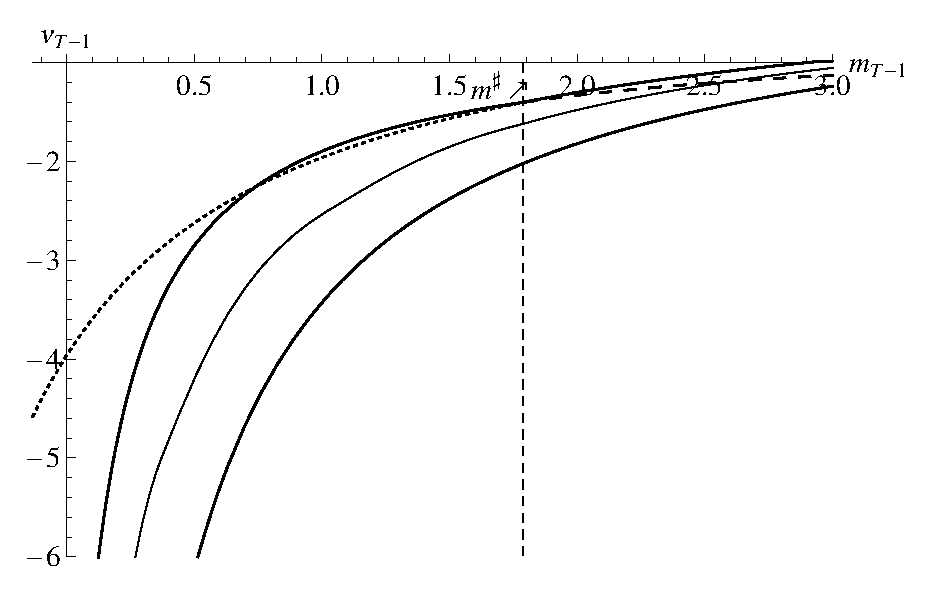
\includegraphics{./Figures/IntExpFOCInvPesReaOptNeed45ValuePlot}
        \caption{A Constrained Optimist's Value Function as Another Upper Bound}
        \label{fig:IntExpFOCInvPesReaOptNeed45ValuePlot}
\end{figure}

\end{comment}

\newcommand{\mtCusp}{\ensuremath{\mRat_{t}^{\#}}}
%\newcommand{\aboveMin \mtCusp}{\ensuremath{\aboveMin \mRat_{t}^{\#}}}

Defining $\mtCusp$ as the `cusp' point where the two upper bounds
intersect:
\begin{eqnarray*}
\left(\aboveMin \mtCusp+\aboveMin \hEnd_{t}\right)\MinMPC_{t} &=& \MaxMPC_{t} \aboveMin \mtCusp \\
\aboveMin \mtCusp &=& \frac{\MinMPC_{t}\aboveMin \hEnd_{t}}{(1-\MinMPC_{t})\MaxMPC_{t}} \\
\mtCusp &=& \frac{\MinMPC_{t}\hEnd_{t}-\hEndMin_{t}}{(1-\MinMPC_{t})\MaxMPC_{t}},
\end{eqnarray*}

  we want to construct a consumption function for $m_{\prdt} \in (\Min{m}_{\prdt}, \mtCusp]$ that respects the
  tighter upper bound:
  \begin{center}
    \begin{tabular}{rcl}
      $ \aboveMin \mNrm_{\prdt} \MPCmin_{\prdt} < $ & $ \cFunc_{\prdt}(\Min{m}_{\prdt}+\aboveMin \mNrm_{\prdt}) $ & $< \MPCmax_{\prdt} \aboveMin \mNrm_{\prdt} $
      % \\  $-\aboveMin \mNrm_{\prdt} \MPCmin_{\prdt} > $ & $ -\cFunc_{\prdt}(\Min{m}_{\prdt}+\aboveMin \mNrm_{\prdt}) $ & $> -\aboveMin \mNrm_{\prdt} $
      \\  $ \aboveMin \mNrm_{\prdt}(\MPCmax_{\prdt}- \MPCmin_{\prdt}) > $ & $ \MPCmax_{\prdt} \aboveMin \mNrm_{\prdt}-\cFunc_{\prdt}(\Min{m}_{\prdt}+\aboveMin \mNrm_{\prdt}) $ & $> 0$
      \\  $1 > $ & $ \left(\frac{\MPCmax_{\prdt} \aboveMin \mNrm_{\prdt}-\cFunc_{\prdt}(\Min{m}_{\prdt}+\aboveMin \mNrm_{\prdt})}{\aboveMin \mNrm_{\prdt}(\MPCmax_{\prdt}- \MPCmin_{\prdt})}\right) $ & $> 0$.
    \end{tabular}
  \end{center}

  Again defining $\mu_{t} =\log \aboveMin \mNrm_{t}$, the object in the middle of the inequality is
  \begin{equation*}\begin{gathered}\begin{aligned}
        \Lo{\koppa}_{t}(\mu_{t})  & \equiv  \frac{\MPCmax_{t}-\cFunc_{t}(\ushort{m}_{t}+e^{\mu_{t}})e^{-\mu_{t}}}{\MPCmax_{t}-\MPCmin_{t}} \label{eq:koppaL}
        \MPCMatch{\\ \Lo{\koppa}^{\mu}_{t}(\mu_{t})  & = \frac{\cFunc_{t}(\ushort{m}_{t}+e^{\mu_{t}})e^{-\mu_{t}}-\MPCFunc_{t}^{m}(\ushort{m}_{t}+e^{\mu_{t}})}{\MPCmax_{t}-\MPCmin_{t}}}{} .
      \end{aligned}\end{gathered}\end{equation*}

As $m_{t}$ approaches
$-\ushort{m}_{t}$, $\Lo{\koppa}_{t}(\mu_{t})$ converges to zero, while as $m_{t}$
approaches $+\infty$, $\Lo{\koppa}_{t}(\mu_{t})$ approaches $1$.

As before (in equation \eqref{eq:vEndtdefn}), we can derive an approximated consumption function; call it
$\Alt{\Lo{\cFunc}}_{t}$.  This function will clearly do a better job approximating the consumption
function for low values of $\mRat_{t}$ while the previous approximation will perform better
for high values of $\mRat_{t}$.

For middling values of $\mRat$ it is not clear which of these
functions will perform better.  However, an alternative is available
which performs well.  Define the highest gridpoint below $\mtCusp$ as
$\bar{\check{\mRat}}_{t}^{\#}$ and the lowest gridpoint above $\mtCusp$ as
$\ushort{\hat{\mRat}}_{t}^{\#}$.  Then there will be a unique interpolating
polynomial that matches the level and slope of the consumption function
at these two points.  Call this function $\tilde{\cFunc}_{t}(\mRat)$.

Using indicator functions that are zero everywhere except for specified intervals,

  \begin{equation*}\begin{gathered}\begin{aligned}
        \vctr{1}_{\text{Lo}}(\mNrm)  & = 1 \text{~if $          \mNrm \leq  \bar{\check{\mNrm}}_{\prdt}^{\#} \phantom{< \mNrm <   \Min{\hat{\mNrm}}_{\prdt}^{\#}          \leq \mNrm}$}
        \\  \vctr{1}_{\text{Mid}}(\mNrm)  & = 1 \text{~if $\phantom{ \mNrm \leq}~ \bar{\check{\mNrm}}_{\prdt}^{\#}          < \mNrm <   \Min{\hat{\mNrm}}_{\prdt}^{\#} \phantom{\leq \mNrm}$}
        \\  \vctr{1}_{\text{Hi}}(\mNrm)  & = 1 \text{~if $\phantom{ \mNrm \leq  ~\bar{\check{\mNrm}}_{\prdt}^{\#}          < \mNrm < } \Min{\hat{\mNrm}}_{\prdt}^{\#}           \leq \mNrm$}
      \end{aligned}\end{gathered}\end{equation*}
  we can define a well-behaved approximating consumption function
  \begin{equation}\begin{gathered}\begin{aligned}
        \Aprx{\cFunc}_{\prdt}  & = \vctr{1}_{\text{Lo}} \Aprx{\Min{\cFunc}}_{\prdt} + \vctr{1}_{\text{Mid}} \Aprx{\tilde{\cFunc}}_{\prdt}+\vctr{1}_{\text{Hi}} \Aprx{\Max{\cFunc}}_{\prdt}.
        %
        \UnifiedNote{[no direct counterpart] (computational: piecewise consumption approximation combining low/mid/high regions)}
      \end{aligned}\end{gathered}\end{equation}

  This just says that, for each interval, we use the approximation that
  is most appropriate.  The function is continuous and
  once-differentiable everywhere, and is therefore well behaved for
  computational purposes.
  \begin{comment}
    In practice, in our problem the difference due to this refinement is displayed in Figure \ref{fig:IntExpFOCInvPesReaOpt45GapPlot}.
    \hypertarget{IntExpFOCInvPesReaOpt45GapPlot}{}
    \begin{figure}
      \includegraphics[width=6in]{./Figures/IntExpFOCInvPesReaOpt45GapPlot}
      \caption{Difference Between $\Aprx{\Hi{\cFunc}}_{L, T-1}$ and $\Aprx{\Hi{\cFunc}}_{H,T-1}$ is Small}
      \label{fig:IntExpFOCInvPesReaOpt45GapPlot}
    \end{figure}
  \end{comment}

  We now construct an upper-bound value function implied for a consumer whose spending behavior is consistent with the refined upper-bound consumption rule.

  For $\mNrm_{\prd} \geq \mNrm_{\prd}^{\#}$, this consumption rule is the same as before,
  so the constructed upper-bound value function is also the same.  However, for
  values $\mNrm_{\prd} < \mNrm_{\prd}^{\#}$ matters are slightly more complicated.

  Start with the fact that at the cusp point,
  \begin{equation*}\begin{gathered}\begin{aligned}
        \bar{\vFunc}_{\prd}(\mtCusp)  & = \uFunc(\bar{\cNrm}_{\prd}(\mtCusp))\PDVCoverc_{\prd}^{T} \\
        & =  \uFunc(\aboveMin \mtCusp  \MPCmax_{\prd})\PDVCoverc_{\prd}^{T}
        .
      \end{aligned}\end{gathered}\end{equation*}

  But for \textit{all} $\mNrm_{\prd}$,
  \begin{equation*}\begin{gathered}\begin{aligned}
        \bar{\vFunc}_{\prd}(\mNrm)  & = \uFunc(\bar{\cNrm}_{\prd}(\mNrm))+ \bar{\vEnd}(\mNrm-\bar{\cNrm}_{\prd}(\mNrm)),
      \end{aligned}\end{gathered}\end{equation*}
  and we assume that for the consumer below the cusp point consumption is given by $\MPCmax \aboveMin \mNrm_{\prd}$ so for $\mNrm_{\prd}< \mtCusp$
  \begin{equation*}\begin{gathered}\begin{aligned}
        \bar{\vFunc}_{\prd}(\mNrm)  & = \uFunc( \MPCmax_{\prd} \aboveMin \mNrm)+ \bar{\vEnd}((1-\MPCmax_{\prd})\aboveMin \mNrm),
      \end{aligned}\end{gathered}\end{equation*}
  which is easy to compute because $\bar{\vEnd}(\aNrm_{\prd}) = \DiscFac \bar{\vFunc}_{\prd+1}(\aNrm_{\prd}\RNrm+1)$
  where $\bar{\vFunc}_{\prd}$ is as defined above because a consumer who ends the current period with assets exceeding
  the lower bound will not expect to be constrained next period.  (Recall again that we are merely constructing an object that is guaranteed to be an \textit{upper bound} for the value that the `realist' consumer will experience.)  At the gridpoints defined by the solution of the
  consumption problem can then construct
  \begin{equation*}\begin{gathered}\begin{aligned}
        \bar{\vInv}_{\prd}(\mNrm)  & = ((1-\CRRA)\bar{\vFunc}_{\prd}(\mNrm))^{1/(1-\CRRA)}
      \end{aligned}\end{gathered}\end{equation*}
  \MPCMatch{and its derivatives}{} which yields the appropriate vector for constructing $\check{\Chi}$ and $\check{\Koppa}$.  The rest of the procedure is analogous to that performed for the consumption rule and is thus omitted for brevity.



\begin{figure}
  \includegraphics[width=6in]{./Figures/IntExpFOCInvPesReaOptNeed45Plot}
\end{figure}

\IfRiskyR{
  \hypertarget{stochastic-rate-of-return}{}
  \subsection{Stochastic Rate of Return}
  \input{cctwMoM/StochasticR-Intro.tex} 

  The easiest case is where the interest factor is i.i.d.,   \begin{equation}\begin{gathered}\begin{aligned}
        \log \Risky_{\prdt+n} & \sim \Nrml(\rfree + \eprem - \sigma^{2}_{\risky}/2,\sigma^{2}_{\risky}) ~\forall~n>0 \label{eq:distRisky}
        %
        \UnifiedNote{defines distribution of R̃ (risky return shock process, IID)}
      \end{aligned}\end{gathered}\end{equation}
 \noindent because in this case \cite{merton:restat} and \cite{samuelson:portfolio} showed that for a consumer without labor income (or with perfectly forecastable labor income) the consumption function is linear, with an MPC.\footnote{See \handoutC{CRRA-RateRisk} for a derivation.}
  \begin{eqnarray}
  \MPC & = & 1- \left(\Discount  \Ex_{t}[\Risky_{t+1}^{1-\CRRA}]\right)^{1/\CRRA} \label{eq:MPCExact}
\end{eqnarray}
and in this case the previous analysis applies once we substitute this MPC for the one that characterizes
the perfect foresight problem without rate-of-return risk.
 
  The more realistic case where the interest factor has some serial correlation is more complex.  We consider
the simplest case that captures the main features of empirical interest rate dynamics: An AR(1) process.  Thus
the specification is
\begin{eqnarray}
  \risky_{t+1}-\risky & = & (\risky_{t}-\risky) \gamma + \epsilon_{t+1}
\end{eqnarray}
where $\risky$ is the long-run mean log interest factor, $0 < \gamma < 1$ is the AR(1) serial correlation
coefficient, and $\epsilon_{t+1}$ is the stochastic shock.

The consumer's problem in this case now has two state variables, $\mRat_{t}$ and $\risky_{t}$, and
is described by
\begin{eqnarray}
        {\vFunc}_{t}({m}_{t},\risky_{t}) & = & \max_{{c}_{t}} ~ \util({c}_{t})+
        \Ex_{t}[{\Discount}_{t+1}\PGro_{t+1}^{1-\CRRA}{\vFunc}_{t+1}({m}_{t+1},\risky_{t+1})] \label{vtNormRisky}
\\         & \text{s.t.} &   \nonumber \\
    {a}_{t}   & = & {m}_{t}-{c}_{t} \nonumber
\\      \risky_{t+1}-\risky & = & (\risky_{t}-\risky)\gamma + \epsilon_{t+1} \notag
\\      \Risky_{t+1} & = & \exp(\risky_{t+1}) \notag
\\      {m}_{t+1} & = & \underbrace{\left(\Risky_{t+1}/\PGro_{t+1}\right)}_{\equiv \Rprod_{t+1}}{a}_{t}+\tShkEmp_{t+1} \nonumber.
\end{eqnarray}

% Kiichi: I will need you to read the literature and figure out how exactly we want to choose the Markov points and transition probabilities.
% When done, you will fill in the [how] text below.

We approximate the AR(1) process by a Markov transition matrix using standard techniques.  The stochastic interest factor is allowed to take
on 11 values centered around the steady-state value $\risky$ and chosen [how?].  Given this Markov transition matrix,
{\it conditional} on the Markov AR(1) state the consumption functions for the `optimist' and the `pessimist' will still be linear,
with identical MPC's that are computed numerically.  Given these MPC's, the (conditional) realist's consumption function can be computed for each Markov state, and the converged consumption rules constitute the solution contingent on the dynamics of the stochastic
interest rate process.

In principle, this refinement should be combined with the previous one;
further exposition of this combination is omitted here because no new
insights spring from the combination of the two techniques.

 
}{}

% \subsection{Habits}

\hypertarget{conclusion}{}
\section{Conclusion}

The method proposed here is not universally applicable.  For example, the method cannot be used for problems for which upper and lower bounds to the `true' solution are not known.  But many problems do have obvious upper and lower bounds, and in those cases (as in the consumption example used in the paper), the method may result in substantial improvements in accuracy and stability of solutions.

\vfill\clearpage
\notinsubfile{\input{.resources/latex/bibliography-blend}} \end{document}\endinput

% Local Variables:
% TeX-master-file: t
% eval: (setq TeX-command-list  (assq-delete-all (car (assoc "BibTeX" TeX-command-list)) TeX-command-list))
% eval: (setq TeX-command-list  (assq-delete-all (car (assoc "Biber"  TeX-command-list)) TeX-command-list))
% eval: (setq TeX-command-list  (remove '("BibTeX" "%(bibtex) %s"    TeX-run-BibTeX nil t :help "Run BibTeX") TeX-command-list))
% eval: (setq TeX-command-list  (remove '("BibTeX"    "bibtex %s"    TeX-run-BibTeX nil (plain-tex-mode latex-mode doctex-mode ams-tex-mode texinfo-mode context-mode)  :help "Run BibTeX") TeX-command-list))
% eval: (setq TeX-command-list  (remove '("BibTeX" "bibtex %s"    TeX-run-BibTeX nil t :help "Run BibTeX") TeX-command-list))
% eval: (add-to-list 'TeX-command-list '("BibTeX" "bibtex %s" TeX-run-BibTeX nil t                                                                              :help "Run BibTeX") t)
% eval: (add-to-list 'TeX-command-list '("BibTeX" "bibtex %s" TeX-run-BibTeX nil (plain-tex-mode latex-mode doctex-mode ams-tex-mode texinfo-mode context-mode) :help "Run BibTeX") t)
% TeX-PDF-mode: t
% TeX-file-line-error: t
% TeX-debug-warnings: t
% LaTeX-command-style: (("" "%(PDF)%(latex) %(file-line-error) %(extraopts) -output-directory=. %S%(PDFout)"))
% TeX-source-correlate-mode: t
% TeX-parse-self: t
% TeX-parse-all-errors: t
% eval: (cond ((string-equal system-type "darwin") (progn (setq TeX-view-program-list '(("Skim" "/Applications/Skim.app/Contents/SharedSupport/displayline -b %n %o %b"))))))
% eval: (cond ((string-equal system-type "gnu/linux") (progn (setq TeX-view-program-list '(("Evince" "evince --page-index=%(outpage) %o"))))))
% eval: (cond ((string-equal system-type "gnu/linux") (progn (setq TeX-view-program-selection '((output-pdf "Evince"))))))
% End:
